\qns{Visualizing Stability}

In this problem, we will explore how the eigenvalues of the system impact how the state changes over time. We already know that stable eigenvalues cause any disturbance in the state or initial condition to decay over time, and unstable eigenvalues cause the magnitude of the state to become unbounded. Also, "marginally (un)stable" eigenvalues cause any disturbance to persist, that is, neither decay nor grow. Recall that a system is stable in continuous time if all eigenvalues have a negative real component, and stable in discrete time if all eigenvalues have a magnitude less than 1.

Where an eigenvalue lies on the complex plane also determines how the state evolves over time. Whether or not a system has complex eigenvalues does not change the end behavior, but it does determine whether the state oscillates (in continuous time) or rotates (in discrete time). 

\textit{For all of the systems shown below, we assume an initial state of $\vec{x}(0) = 0$.}
\newline

\textbf{Continuous Time Systems}:

\begin{tabular}{|p{0.33\textwidth}| p{0.33\textwidth}|p{0.33\textwidth}|} 
    \hline
    A & B & C \\
        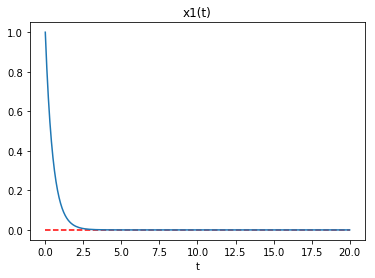
\includegraphics[width = 0.33 \textwidth]{\bank/stability/figures/continuous-graphs/real_negative_x1.png} &
        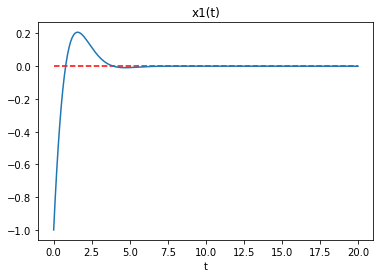
\includegraphics[width = 0.33 \textwidth]{\bank/stability/figures/continuous-graphs/complex_negative_x1.png} &
        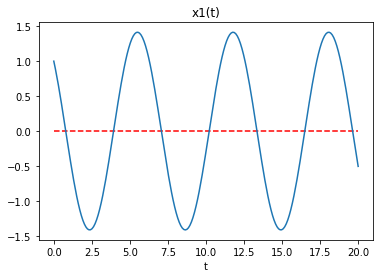
\includegraphics[width = 0.33 \textwidth]{\bank/stability/figures/continuous-graphs/imaginary_x1.png} \\
        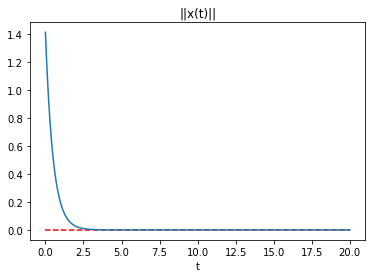
\includegraphics[width = 0.33 \textwidth]{\bank/stability/figures/continuous-graphs/real_negative_mag.png} &
        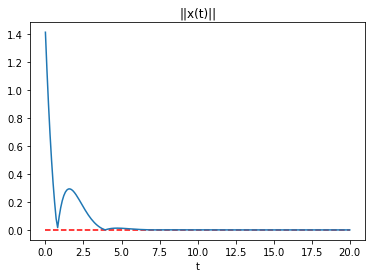
\includegraphics[width = 0.33 \textwidth]{\bank/stability/figures/continuous-graphs/complex_negative_mag.png} &
        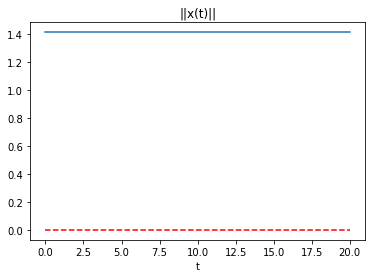
\includegraphics[width = 0.33 \textwidth]{\bank/stability/figures/continuous-graphs/imaginary_mag.png} \\
    \hline
\end{tabular}

\begin{tabular}{|p{0.33\textwidth}| p{0.33\textwidth}|p{0.33\textwidth}|} 
    \hline
    D & E & F \\
        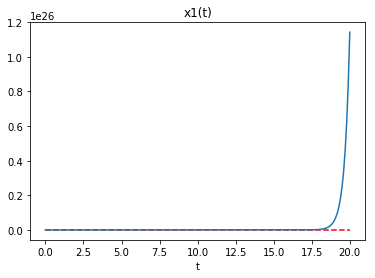
\includegraphics[width = 0.33 \textwidth]{\bank/stability/figures/continuous-graphs/real_positive_x1.png} &
        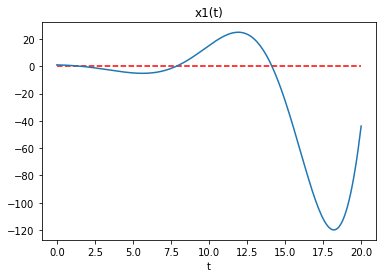
\includegraphics[width = 0.33 \textwidth]{\bank/stability/figures/continuous-graphs/complex_positive_x1.png} &
        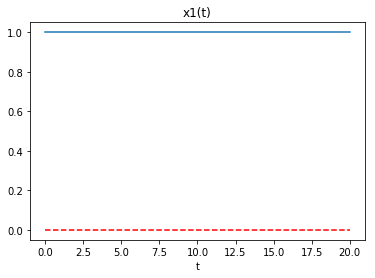
\includegraphics[width = 0.33 \textwidth]{\bank/stability/figures/continuous-graphs/zero_x1.png} \\
        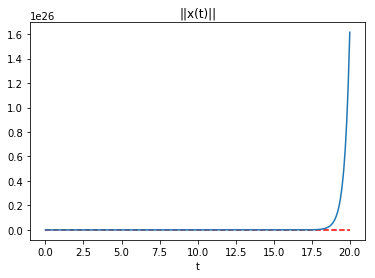
\includegraphics[width = 0.33 \textwidth]{\bank/stability/figures/continuous-graphs/real_positive_mag.png} &
        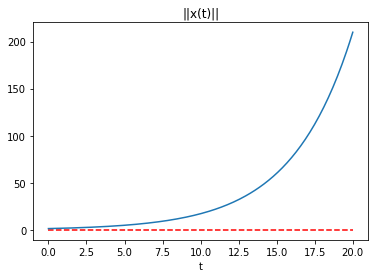
\includegraphics[width = 0.33 \textwidth]{\bank/stability/figures/continuous-graphs/complex_positive_mag.png} &
        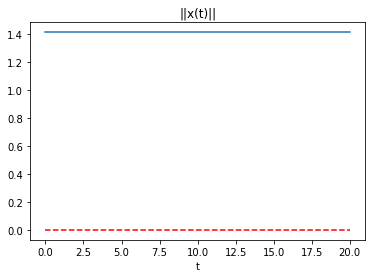
\includegraphics[width = 0.33 \textwidth]{\bank/stability/figures/continuous-graphs/zero_mag.png} \\
        \hline
\end{tabular}

\begin{enumerate}
    \qitem Consider the system
    \begin{align*}
        \frac{d}{dt} \vec{x}(t) = \begin{bmatrix}
            0 & -1 \\
            1 & 0
        \end{bmatrix} \vec{x}(t)
    \end{align*}
    with eigenvalues $\lambda = \pm j$.
    \begin{enumerate}
        \item What type of eigenvalues does this system have (eg. real and positive, real and negative, imaginary, complex)?
        \sol {
            This system has purely imaginary eigenvalues.
        }
        \item Is this system stable? Why?
        \sol {
            The system is marginally (un)stable because $\operatorname{Re}(\lambda_i) = 0$.
        }
        \item Which of the above graphs could represent this system?
        \sol {
            C. The magnitude of the state stays constant because the system has eigenvalues of magnitude 1, and the first state element oscillates due to the imaginary eigenvalues.
        }
    \end{enumerate}

    \qitem Consider the system
    \begin{align*}
        \frac{d}{dt} \vec{x}(t) = \begin{bmatrix}
            2 & 1 \\
            1 & 2
        \end{bmatrix} \vec{x}(t)
    \end{align*}
    with eigenvalues $\lambda = 3, 1$.
    \begin{enumerate}
        \item What type of eigenvalues does this system have (eg. real and positive, real and negative, imaginary, complex)?
        \sol {
            This system has real eigenvalues which are both positive.
        }
        \item Is this system stable? Why?
        \sol {
            The system is unstable because both eigenvalues have a positive real component.
        }
        \item Which of the above graphs could represent this system?
        \sol {
            D. The magnitude of the state blows up to infinity as time goes on, since the solutions are real exponentials with positive eigenvalues in the exponent.
        }
    \end{enumerate}

    \qitem Consider the system
    \begin{align*}
        \frac{d}{dt} \vec{x}(t) = \begin{bmatrix}
            -1 & 1 \\
            -1 & -1
        \end{bmatrix} \vec{x}(t)
    \end{align*}
    with eigenvalues $\lambda = -1 \pm j$.
    \begin{enumerate}
        \item What type of eigenvalues does this system have (eg. real and positive, real and negative, imaginary, complex)?
        \sol {
            This system has complex eigenvalues.
        }
        \item Is this system stable? Why?
        \sol {
            $\operatorname{Re}(\lambda_i) < 0$ for both eigenvalues, so the system is stable.
        }
        \item Which of the above graphs could represent this system?
        \sol {
            B. The magnitude of the state decreases exponentially because the system is stable, and the first state element fluctuates up and down (due to the solution to the system of differential equations being linear combinations of sinusoids) because the eigenvalues are complex.
        }
    \end{enumerate}

    \qitem Consider the system
    \begin{align*}
        \frac{d}{dt} \vec{x}(t) = \begin{bmatrix}
            0 & 0 \\
            0 & 0
        \end{bmatrix} \vec{x}(t)
    \end{align*}
    with a repeated eigenvalue $\lambda = 0$.
    \begin{enumerate}
        \item What type of eigenvalues does this system have (eg. real and positive, real and negative, imaginary, complex)?
        \sol {
            This system has a purely real eigenvalue, equal to $0$.
        }
        \item Is this system stable? Why?
        \sol {
            The system is marginally (un)stable because the real component of the eigenvalue is equal to $0$.
        }
        \item Which of the above graphs could represent this system?
        \sol {
            F. The magnitude stays the same, and the state doesn't change. 
        }
    \end{enumerate}

    \qitem Consider the system
    \begin{align*}
        \frac{d}{dt} \vec{x}(t) = \begin{bmatrix}
            \frac{1}{4} & -\frac{1}{2} \\
            \frac{1}{2} & \frac{1}{4}
        \end{bmatrix} \vec{x}(t)
    \end{align*}
    with eigenvalues $\lambda = \frac{1}{4} \pm \frac{1}{2}j$.
    \begin{enumerate}
        \item What type of eigenvalues does this system have (eg. real and positive, real and negative, imaginary, complex)?
        \sol {
            This system has complex eigenvalues, and the real components are both positive.
        }
        \item Is this system stable? Why?
        \sol {
            The system is unstable because at least one eigenvalue (in this case both) has a real component $\geq$ 0.
        }
        \item Which of the above graphs could represent this system?
        \sol {
            E. The magnitude of the state grows exponentially, and the first state oscillates within an envelope due to the complex eigenvalues.
        }
    \end{enumerate}

    \qitem Consider the system
    \begin{align*}
        \frac{d}{dt} \vec{x}(t) = \begin{bmatrix}
            -4 & 2 \\
             2 & -4
        \end{bmatrix} \vec{x}(t)
    \end{align*}
    with eigenvalues $\lambda = -6, -2$.
    \begin{enumerate}
        \item What type of eigenvalues does this system have (eg. real and positive, real and negative, imaginary, complex)?
        \sol {
            This system has purely real eigenvalues, and both are negative.
        }
        \item Is this system stable? Why?
        \sol {
            $\operatorname{Re}(\lambda_i) < 0$ for both eigenvalues, so the system is stable.
        }
        \item Which of the above graphs could represent this system?
        \sol {
            A. The magnitude of the state decreases exponentially because the system is stable, and there is no rotation (the first state element doesn't fluctuate up and down) because the eigenvalues are purely real.
        }
    \end{enumerate}
\end{enumerate}

\newpage
\textbf{Discrete Time Systems}:

The following graphs represent different two-dimensional discrete-time systems with the initial condition $\vec{x}(0) = \begin{bsmallmatrix} 1 & 1 \end{bsmallmatrix}^T$. For each system, the top graph is the first state element over time ($x_1(k)$), and the bottom graph is the magnitude of the state over time ($||\vec{x}(k)||$). \\

\begin{tabular}{|p{0.33\textwidth}| p{0.33\textwidth}|p{0.33\textwidth}|} 
    \hline
    A & B & C \\
        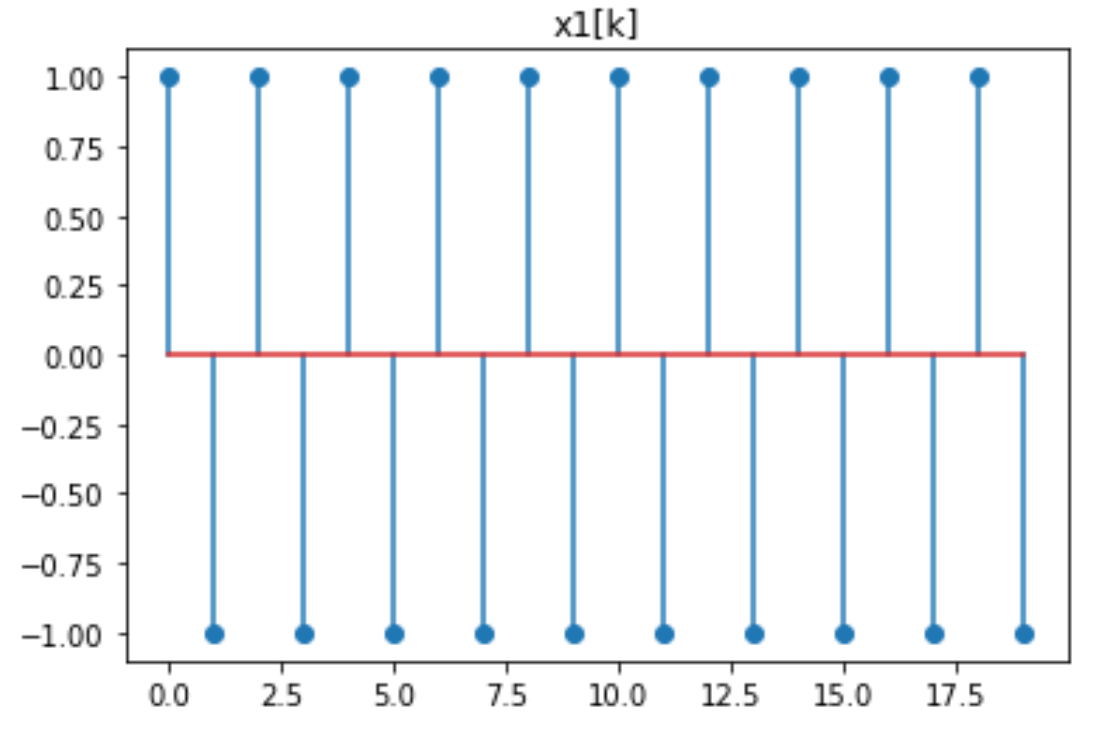
\includegraphics[width = 0.33 \textwidth]{\bank/stability/figures/discrete-graphs/marginal-negative-x1.PNG} &
        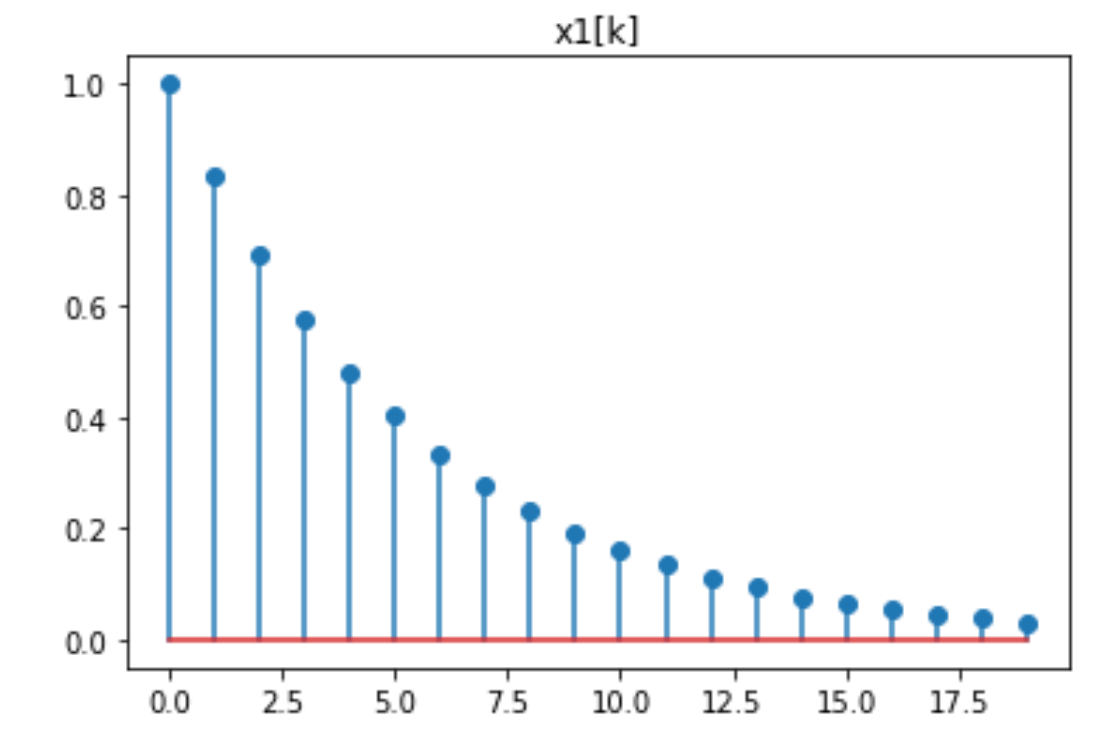
\includegraphics[width = 0.33 \textwidth]{\bank/stability/figures/discrete-graphs/stable-real-x1.PNG} &
        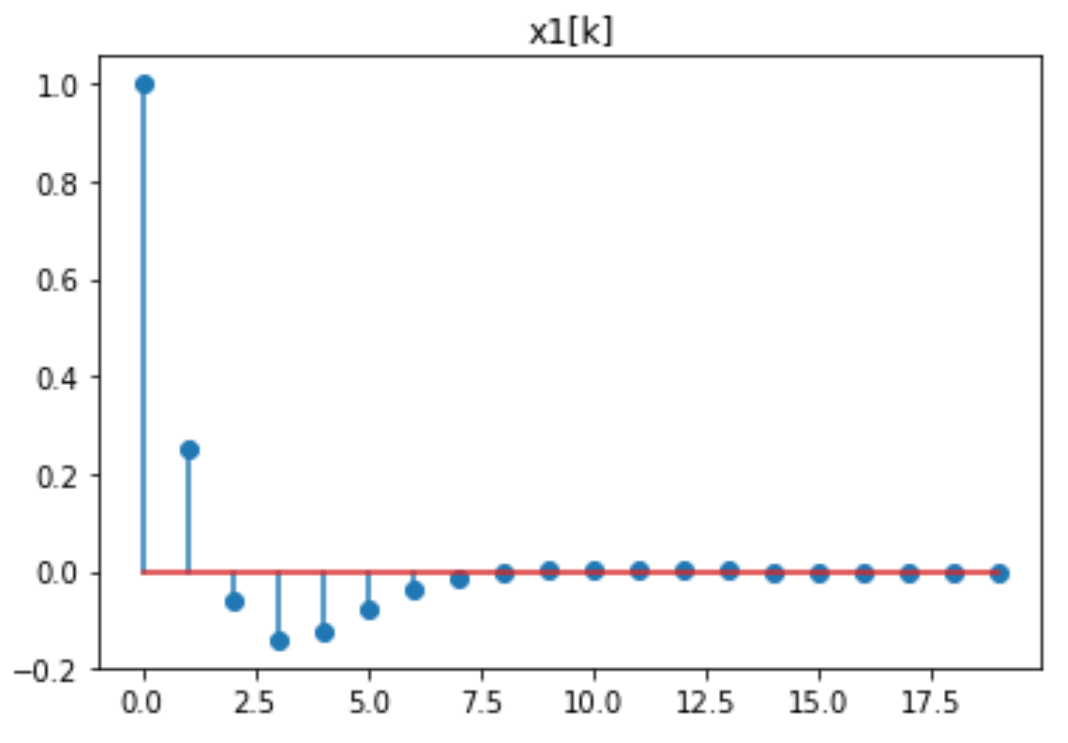
\includegraphics[width = 0.33 \textwidth]{\bank/stability/figures/discrete-graphs/stable-complex-x1.PNG} \\
        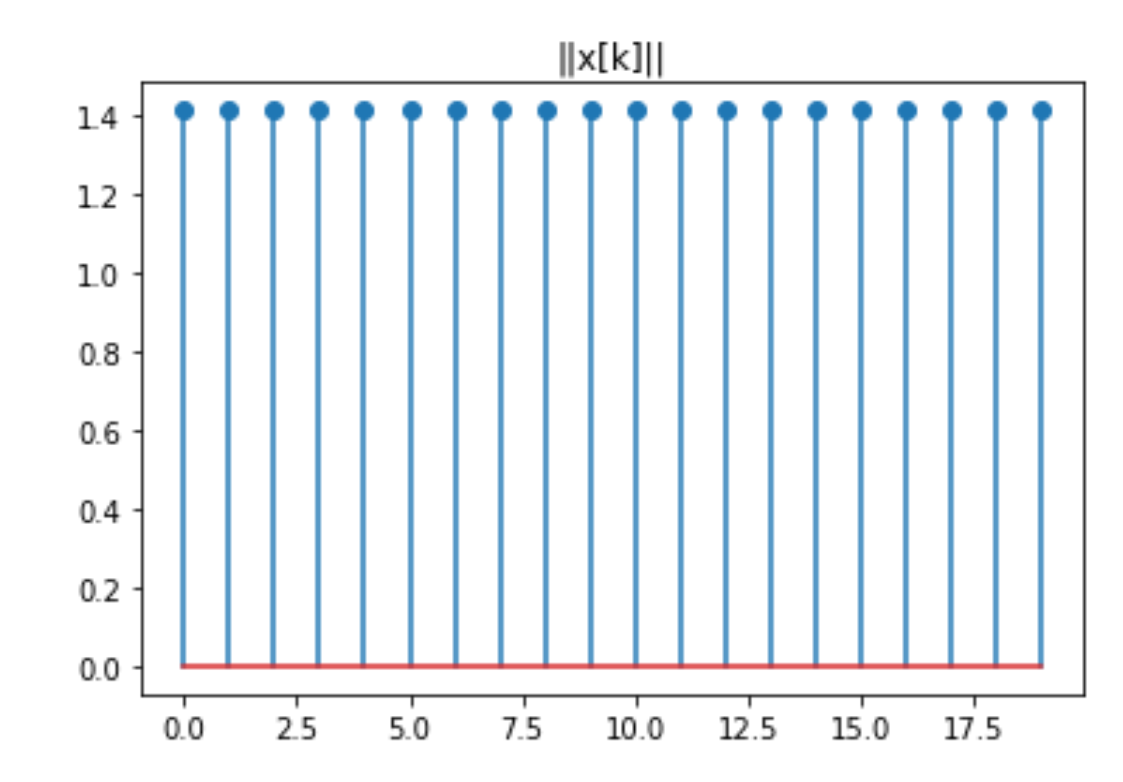
\includegraphics[width = 0.33 \textwidth]{\bank/stability/figures/discrete-graphs/marginal-negative-mag.PNG} &
        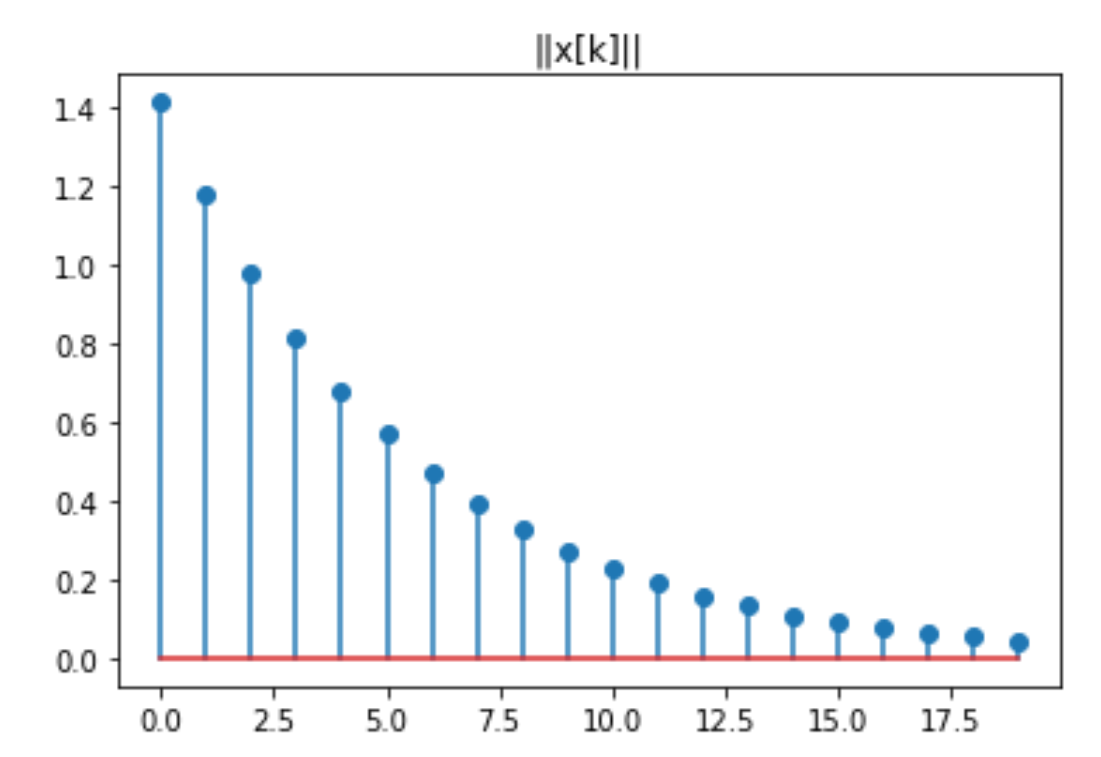
\includegraphics[width = 0.33 \textwidth]{\bank/stability/figures/discrete-graphs/stable-real-mag.PNG} &
        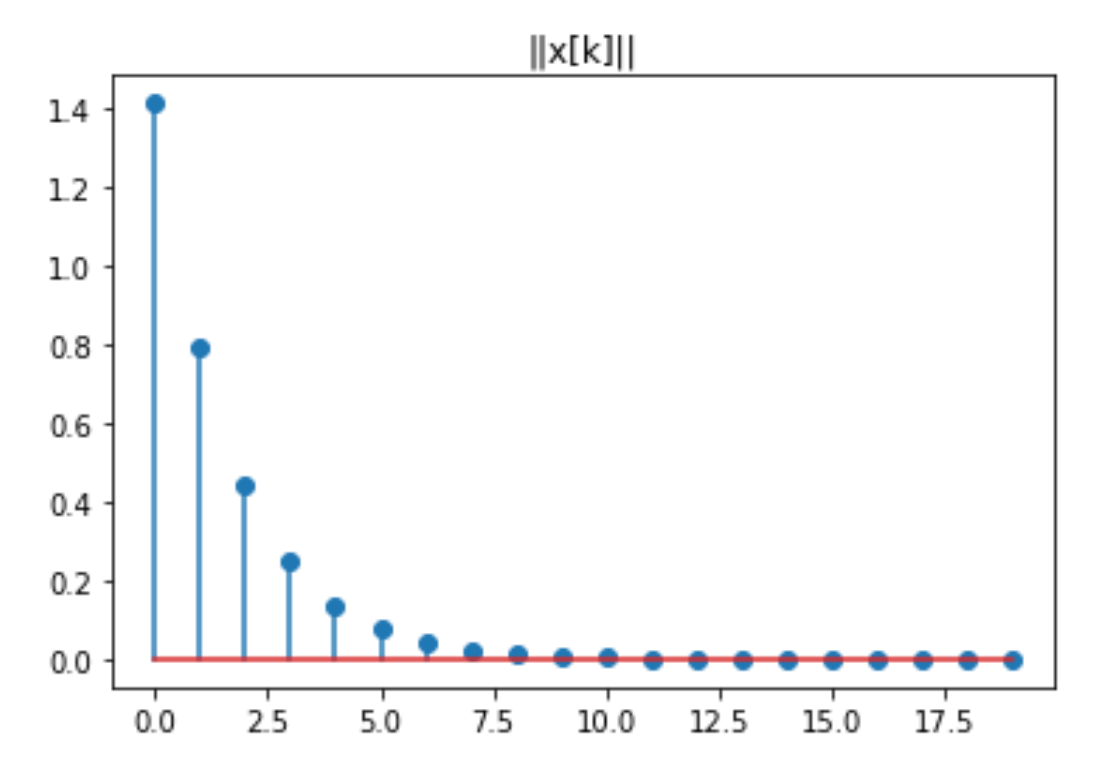
\includegraphics[width = 0.33 \textwidth]{\bank/stability/figures/discrete-graphs/stable-complex-mag.PNG}\\
    \hline
\end{tabular}

\begin{tabular}{|p{0.33\textwidth}| p{0.33\textwidth}|p{0.33\textwidth}|} 
    \hline
    D & E & F \\
        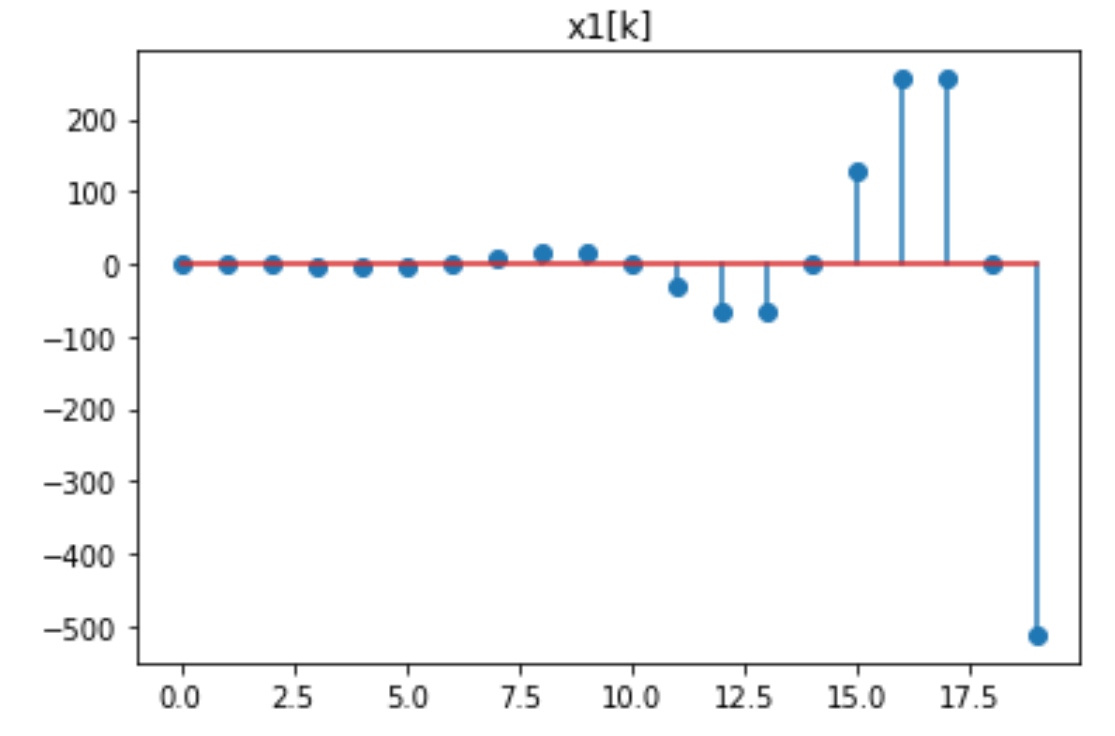
\includegraphics[width = 0.33 \textwidth]{\bank/stability/figures/discrete-graphs/unstable-complex-x1.PNG} &
        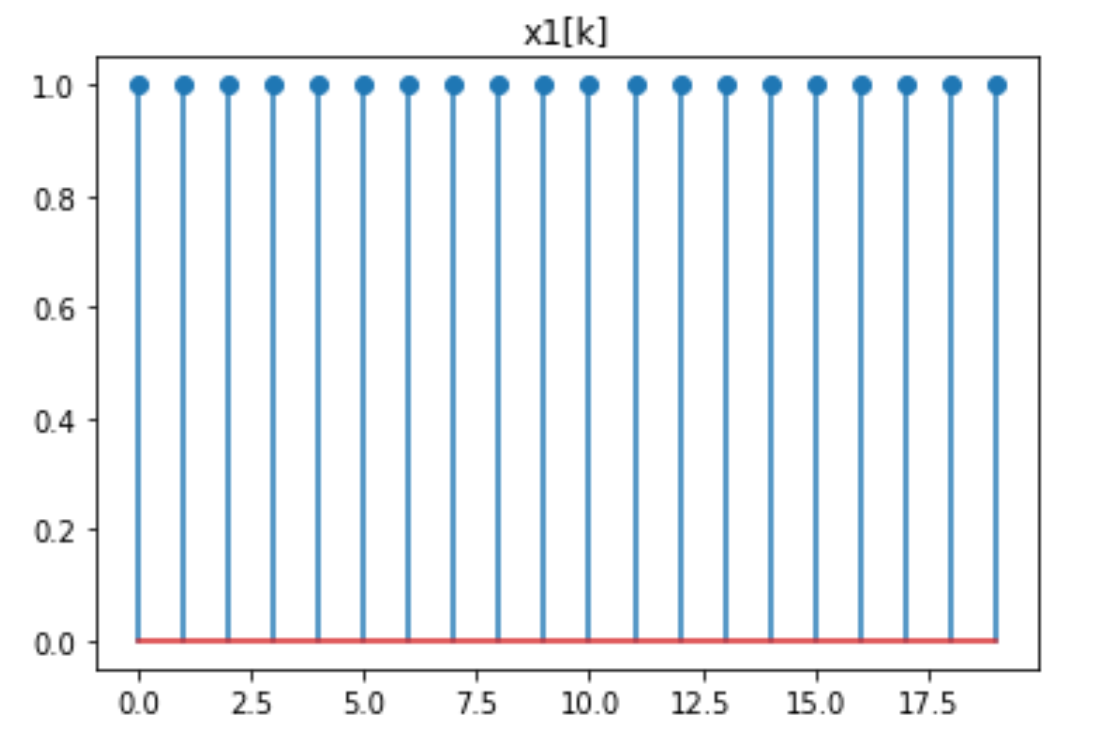
\includegraphics[width = 0.33 \textwidth]{\bank/stability/figures/discrete-graphs/marginal-real-x1.PNG} &
        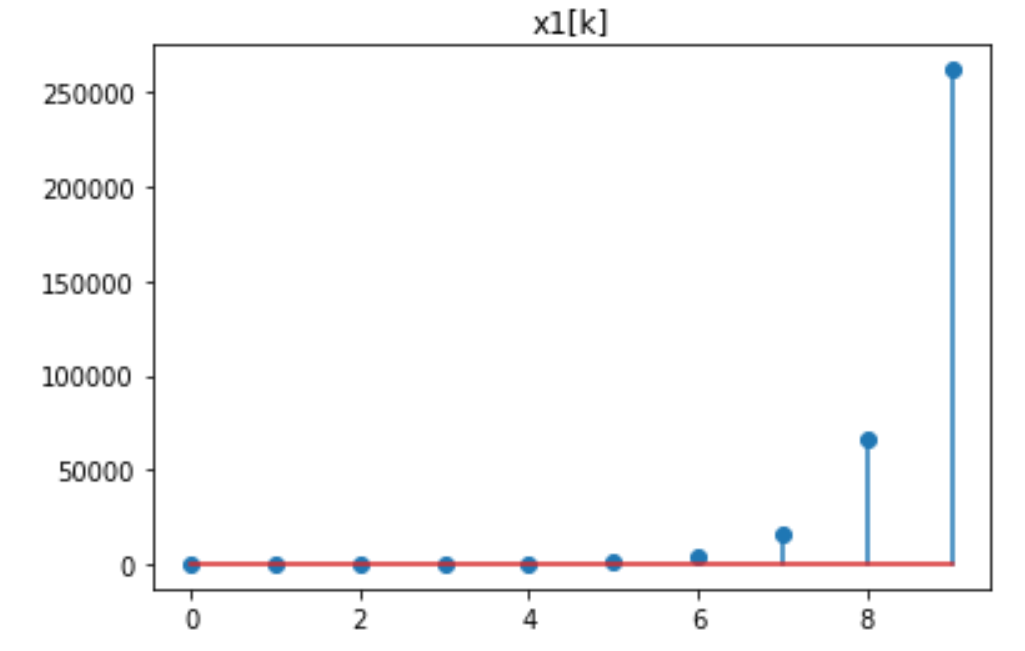
\includegraphics[width = 0.33 \textwidth]{\bank/stability/figures/discrete-graphs/unstable-real-x1.PNG} \\
        
        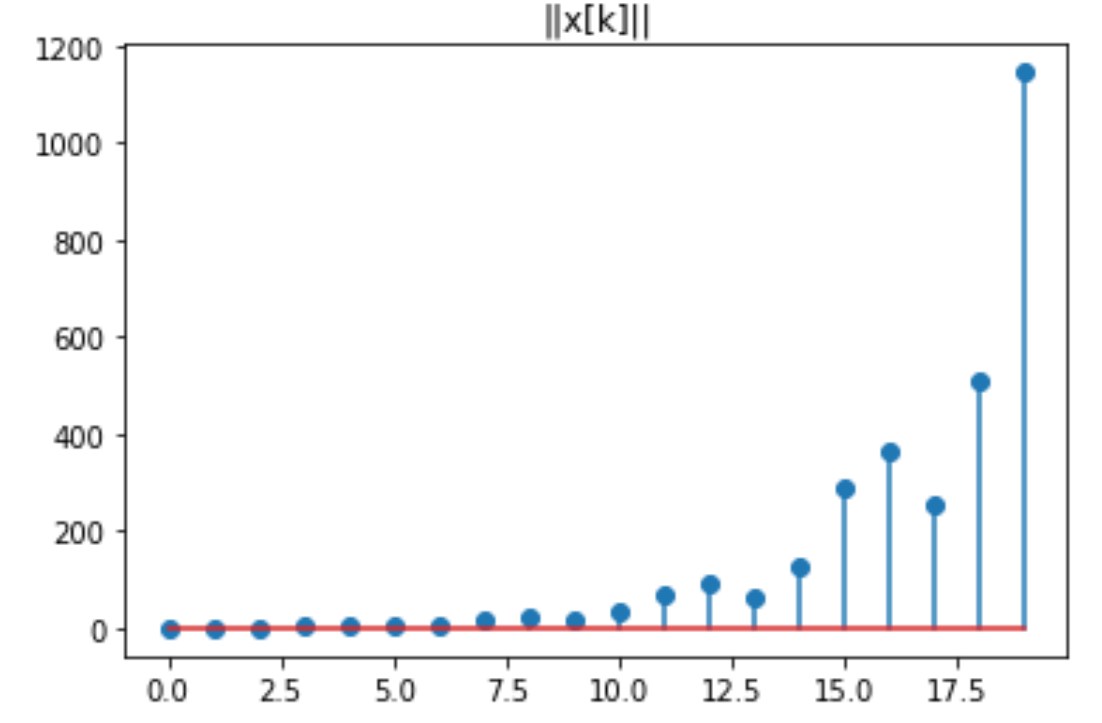
\includegraphics[width = 0.33 \textwidth]{\bank/stability/figures/discrete-graphs/unstable-complex-mag.PNG} &
        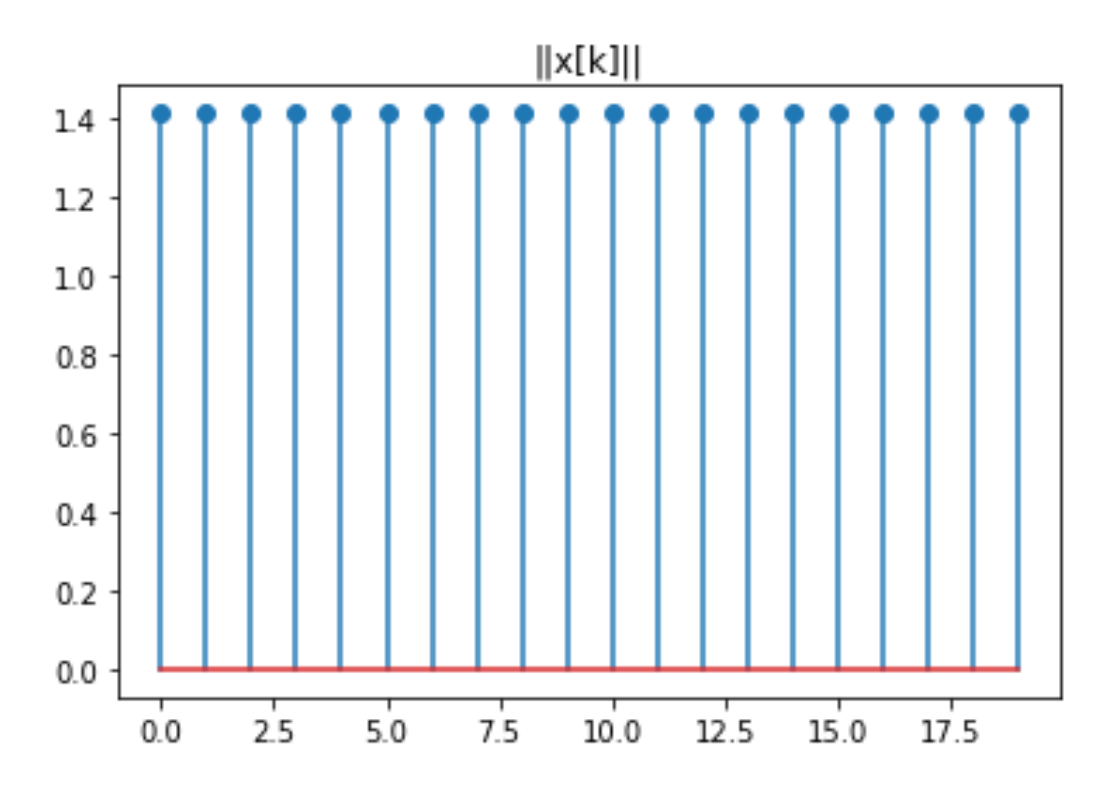
\includegraphics[width = 0.33 \textwidth]{\bank/stability/figures/discrete-graphs/marginal-real-mag.PNG} &
        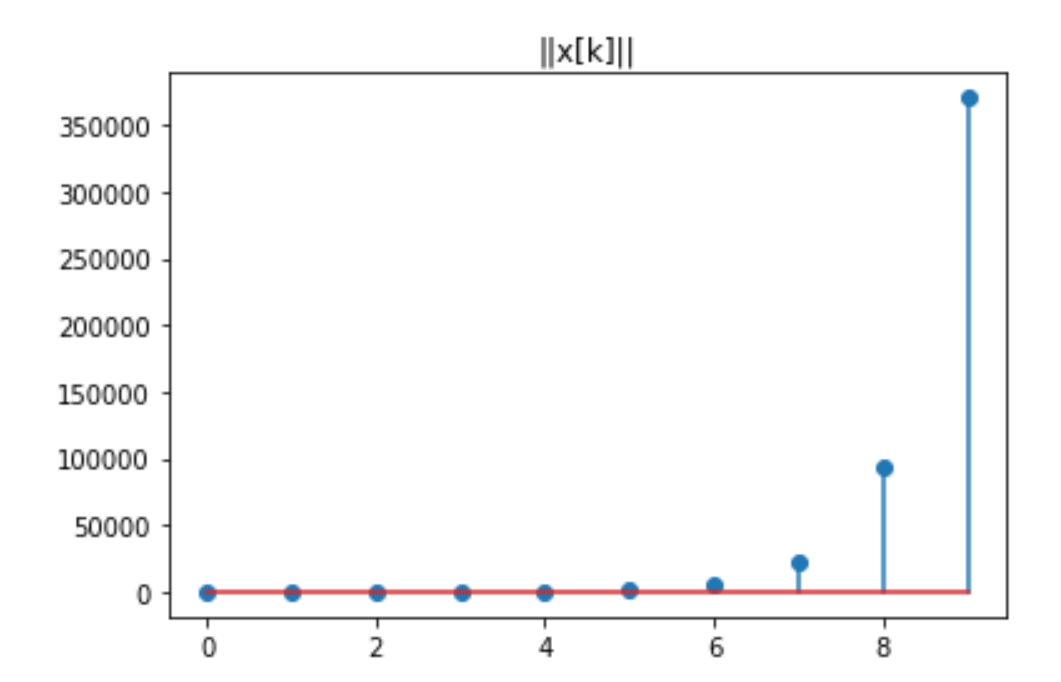
\includegraphics[width = 0.33 \textwidth]{\bank/stability/figures/discrete-graphs/unstable-real-mag.PNG}\\
        \hline
\end{tabular}

\begin{enumerate}
    \qitem Consider the system
    \begin{align*}
        \vec{x}(k + 1) = \begin{bmatrix}
            \frac{1}{2} & \frac{1}{3} \\
            \frac{1}{3} & \frac{1}{2}
        \end{bmatrix} \vec{x}(k)
    \end{align*}
    with eigenvalues $\frac{5}{6}$ and $\frac{1}{6}$.
    \begin{enumerate}
        \item What type of eigenvalues does this system have (eg. real and positive, real and negative, imaginary, complex)?
        \sol {
            This system has purely real eigenvalues, and both are positive.
        }
        \item Is this system stable? Why?
        \sol {
            The magnitude of both eigenvalues is less than 1, so the system is stable.
        }
        \item Which of the above graphs could represent this system?
        \sol {
            B. The magnitude of the state decreases exponentially because the system is stable, and there is no rotation (the first state element doesn't fluctuate up and down) because the eigenvalues are real.
        }
    \end{enumerate}

    \qitem Consider the system
    \begin{align*}
        \vec{x}(k + 1) = \begin{bmatrix}
            \frac{1}{2} & -\frac{1}{4} \\
            \frac{1}{4} & \frac{1}{2}
        \end{bmatrix} \vec{x}(k)
    \end{align*}
    with eigenvalues $\frac{1}{2} \pm \frac{1}{4}j$.
    \begin{enumerate}
        \item What type of eigenvalues does this system have (eg. real and positive, real and negative, imaginary, complex)?
        \sol {
            This system has complex eigenvalues.
        }
        \item Is this system stable? Why?
        \sol {
            The magnitude of both eigenvalues is $\sqrt{(1/2)^2 + (1/4)^2} < 1$, so the system is stable.
        }
        \item Which of the above graphs could represent this system?
        \sol {
            C. The magnitude of the state decreases exponentially because the system is stable, and the first state element fluctuates up and down (due to rotation of the state vector) because the eigenvalues are complex.
        }
    \end{enumerate}

    \qitem Consider the system
    \begin{align*}
        \vec{x}(k + 1) = \begin{bmatrix}
            0 & 1 \\
            -1 & 2
        \end{bmatrix} \vec{x}(k)
    \end{align*}
    with a repeated eigenvalue of 1.
    \begin{enumerate}
        \item What type of eigenvalues does this system have (eg. real and positive, real and negative, imaginary, complex)?
        \sol {
            This system has real eigenvalues, and both are positive.
        }
        \item Is this system stable? Why?
        \sol {
            The system is marginally (un)stable because both eigenvalues have a magnitude of 1.
        }
        \item Which of the above graphs could represent this system?
        \sol {
            E. The magnitude of the state stays constant because the system has eigenvalues of magnitude 1, and the first state element does not switch between positive and negative because both eigenvalues are positive. 
        }
    \end{enumerate}

    \qitem Consider the system
    \begin{align*}
        \vec{x}(k + 1) = \begin{bmatrix}
            -1 & 0 \\
            0 & 1
        \end{bmatrix} \vec{x}(k)
    \end{align*}
    with eigenvalues of -1 and 1.
    \begin{enumerate}
        \item What type of eigenvalues does this system have (eg. real and positive, real and negative, imaginary, complex)?
        \sol {
            This system has real eigenvalues, with one positive and the other negative.
        }
        \item Is this system stable? Why?
        \sol {
            The system is marginally (un)stable because both eigenvalues have a magnitude of 1.
        }
        \item Which of the above graphs could represent this system?
        \sol {
            A. The magnitude of the state stays constant because the system has eigenvalues of magnitude 1, and the eigenvalue of negative 1 results in the first state element switching between positive and negative. Note that only the first state element switches between positive and negative; if we looked at $x_2$, the graph would look like E.
        }
    \end{enumerate}

    \qitem Consider the system
    \begin{align*}
        \vec{x}(k + 1) = \begin{bmatrix}
            1 & 1 \\
            1 & 3
        \end{bmatrix} \vec{x}(k)
    \end{align*}
    with a eigenvalues 2 and 4.
    \begin{enumerate}
        \item What type of eigenvalues does this system have (eg. real and positive, real and negative, imaginary, complex)?
        \sol {
            This system has real eigenvalues, and both are positive.
        }
        \item Is this system stable? Why?
        \sol {
            The system is unstable because at least one eigenvalue (in this case both) has a magnitude greater than 1.
        }
        \item Which of the above graphs could represent this system?
        \sol {
            F. The magnitude of the state grows exponentially because the system is unstable, and the first state element does not switch between positive and negative because both eigenvalues are real and positive. 
        }
    \end{enumerate}

    \qitem Consider the system
    \begin{align*}
        \vec{x}(k + 1) = \begin{bmatrix}
            0 & 1 \\
            -2 & 2
        \end{bmatrix} \vec{x}(k)
    \end{align*}
    with a eigenvalues $1 \pm j$.
    \begin{enumerate}
        \item What type of eigenvalues does this system have (eg. real and positive, real and negative, imaginary, complex)?
        \sol {
            This system has complex eigenvalues.
        }
        \item Is this system stable? Why?
        \sol {
            The system is unstable because at least one eigenvalue (in this case both) has a magnitude greater than 1.
        }
        \item Which of the above graphs could represent this system?
        \sol {
            D. The magnitude of the state grows exponentially because the system is unstable, and the first state element switches between positive and negative because both the eigenvalues are complex. 
        }
    \end{enumerate}
\end{enumerate}
